\subsection{Systeemmodellen}
\subsubsection{Datamodel}
Na een brainstormsessie met alle groepsleden is het volgende model bedacht om de verschillende entiteiten in te delen.
\begin{figure}[htp]
\begin{center}
	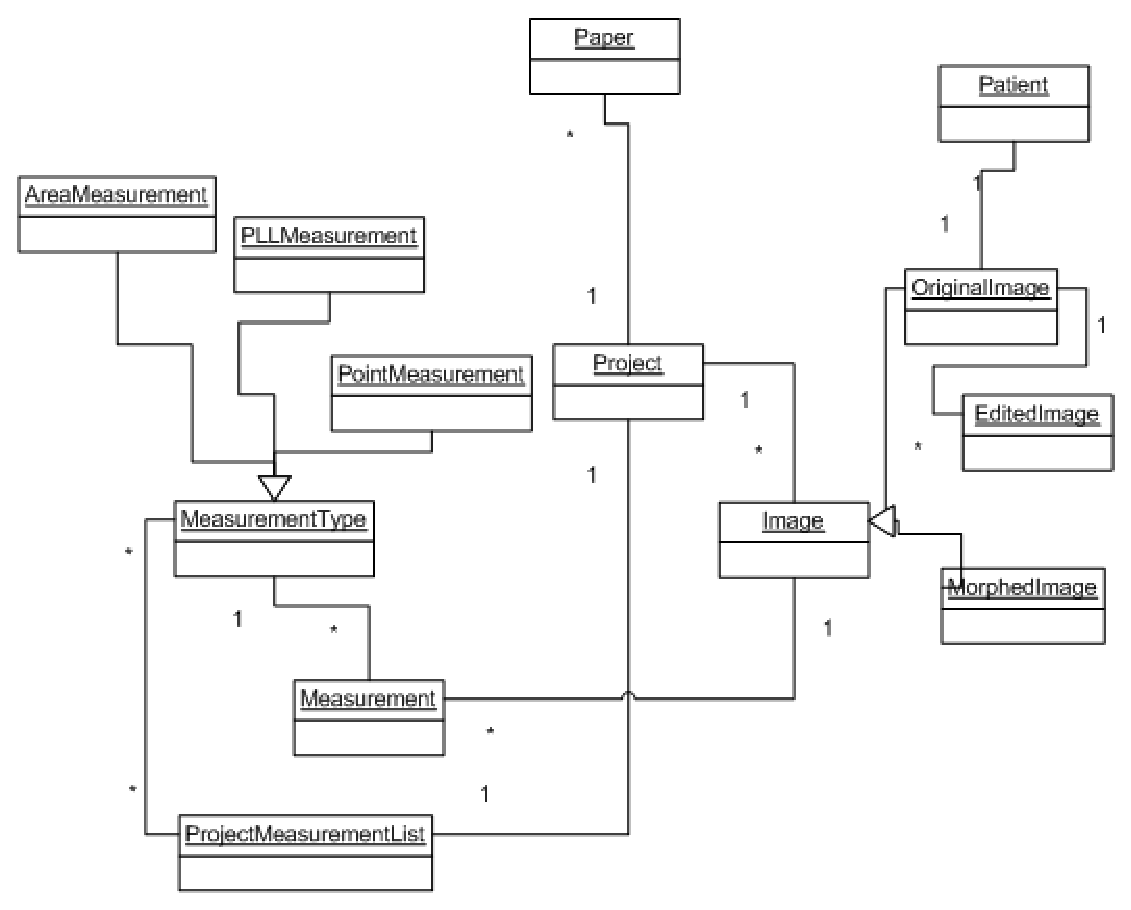
\includegraphics[scale=0.65]{brainstorm_klassediagram}
\caption{Datamodel}
\label{default}
\end{center}
\end{figure}


\section{Scenario's}

%%%%%%%%%%%%%%%%%%%%%%%%%%%%%%%%%%%%%%%%%%%%%%%%%%%%%%%%%%%%%%%%%%%%%%%%%%%%%%%%%%%%%%%%%%%
%% Algemeen
In deze paragraaf beschrijven we twee use cases van gebruikers die het systeem voor verschillend doeleinde willen inzetten.

\begin{enumerate}

\item   Naam: Toevoegen van foto aan project \\
	Actor:
	\begin{itemize}
		\item Anton: Gebruiker met beheerder account
	\end{itemize}
	Flow of events
	\begin{enumerate}
        \item Anton heeft een account als beheerder op het systeem en wil een foto toevoegen. Hij start hiertoe de applicatie op.
        \item Bij het opstarten vraagt het systeem Anton om zijn gebruikersnaam en wachtwoord.
        \item Anton voert zijn gegevens in en klikt op de knop `Inloggen'.
        \item Het systeem logt Anton in en laat de relevante mogelijkheden zien voor zijn gebruikersaccount.
				\item Hij klikt op "foto toevoegen", selecteert een project en selecteert de foto.
				\item Vervolgens voegt Anton meta-data over de foto toe en klikt op 'Toevoegen' 
				\item Het resultaat (toegevoegde foto aan relevante project) wordt getoond.
    \end{enumerate}

\item   Naam: Een gemiddelde foto weergeven \\
	Actor:
	\begin{itemize}
		\item Dr. Kleinrensink: Gebruiker met chirurg account
	\end{itemize}
	Flow of events
	\begin{enumerate}
	\item Dr. Kleinrensink heeft een account als chirurg en wil een gemiddelde foto bekijken.
	\item Nadat hij de applicatie opgestart heeft logt hij in met zijn account.
	\item Hij selecteert 'visualisatie' en kiest het project waar hij de foto van wil zien.
	\item Het systeem laat Dr. Kleinrensink nu de gewenste visualisatie zien.
	\end{enumerate}
\end{enumerate}

